\documentclass[aspectratio=169,11pt]{beamer}

% ============================================================
% Theme
% ============================================================
\usetheme{Madrid}
\usecolortheme{seahorse}
\setbeamertemplate{navigation symbols}{}

% ============================================================
% Encoding (pdfLaTeX-safe)
% ============================================================
\usepackage[utf8]{inputenc}
\usepackage[T1]{fontenc}
\usepackage{lmodern}

% ============================================================
% Packages
% ============================================================
\usepackage{amsmath}
\usepackage{xcolor}
\usepackage{listings}
\usepackage{tikz}
\usetikzlibrary{automata,positioning,arrows.meta}

% ============================================================
% Listings
% ============================================================
\lstset{
	basicstyle=\ttfamily\small,
	frame=single,
	breaklines=true,
	columns=fullflexible,
	keywordstyle=\color{blue},
	commentstyle=\color{gray},
	stringstyle=\color{red},
	showstringspaces=false
}

% ============================================================
% Title
% ============================================================
\title{Concurrency \& Distributed Systems}
\subtitle{Week 2 --- Part 2: Lifecycle States + Scheduling Myths}
\author{Dr. Mohamad Aoude}
\institute{Lebanese University \\ Faculty of Engineering}
\date{\today}

% ============================================================
\begin{document}
	
	% ------------------------------------------------------------
	% Slide 1
	% ------------------------------------------------------------
	\begin{frame}
		\titlepage
	\end{frame}
	
	% ------------------------------------------------------------
	% Slide 2
	% ------------------------------------------------------------
	\begin{frame}{Why This Block Matters}
		\begin{itemize}
			\item Threads are \textbf{state machines}, not “running things”
			\item Debugging hangs = reading \textbf{state transitions}
			\item Performance bottlenecks = \textbf{BLOCKED} and contention
			\item Correctness must not depend on \textbf{timing}
		\end{itemize}
		
		\vspace{4mm}
		\begin{block}{Engineering lens}
			Concurrency failures are often \textbf{scheduler + lock + state} failures.
		\end{block}
	\end{frame}
	
	% ------------------------------------------------------------
	% Slide 3
	% ------------------------------------------------------------
	\begin{frame}{Lifecycle Overview (Java)}
		\begin{itemize}
			\item \textbf{NEW}
			\item \textbf{RUNNABLE}
			\item \textbf{BLOCKED}
			\item \textbf{WAITING}
			\item \textbf{TIMED\_WAITING}
			\item \textbf{TERMINATED}
		\end{itemize}
		
		\vspace{4mm}
		\begin{block}{Key precision}
			RUNNABLE = \textbf{ready OR executing}. Java does not distinguish.
		\end{block}
	\end{frame}
	
	% ------------------------------------------------------------
	% Slide 4 (Enhanced TikZ Diagram)
	% ------------------------------------------------------------
	\begin{frame}{Lifecycle State Diagram}
		\centering
		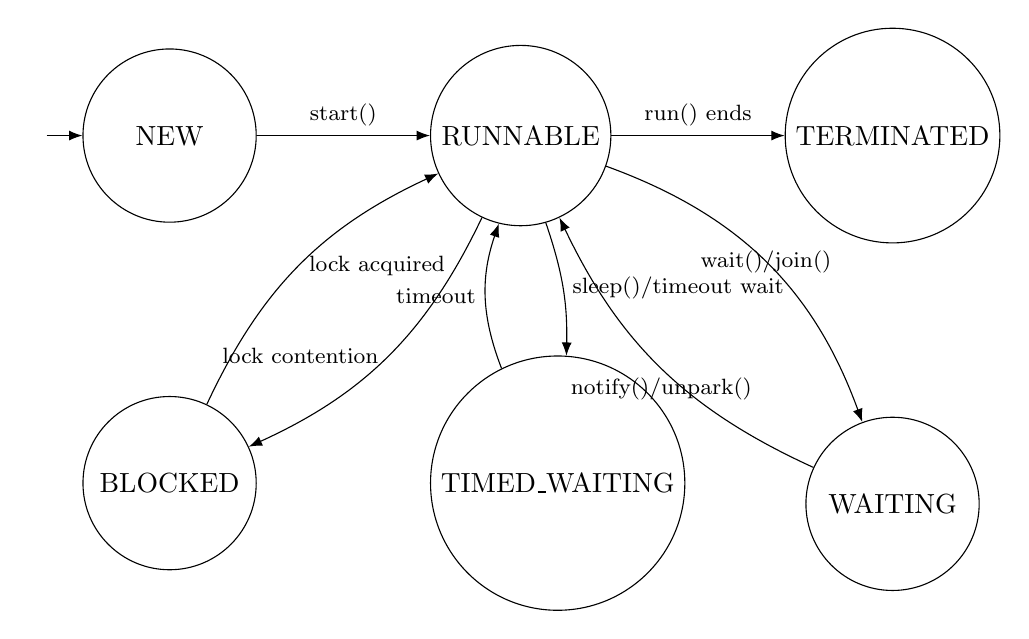
\begin{tikzpicture}[
			>=Latex,
			node distance=2.2cm,
			every state/.style={draw, rounded corners, minimum width=2.2cm, minimum height=0.9cm},
			initial text={}
			]
			\node[state, initial] (new) {NEW};
			\node[state, right=of new] (runnable) {RUNNABLE};
			\node[state, right=of runnable] (term) {TERMINATED};
			\node[state, below=of new] (blocked) {BLOCKED};
			\node[state, below=of term] (waiting) {WAITING};
			\node[state, right=of blocked] (timed) {TIMED\_WAITING};
			
			
			\path[->] (new) edge node[above] {\footnotesize start()} (runnable);
			\path[->] (runnable) edge[bend left=20] node[left] {\footnotesize lock contention} (blocked);
			\path[->] (blocked) edge[bend left=20] node[right] {\footnotesize lock acquired} (runnable);
			
			\path[->] (runnable) edge[bend left=25] node[bend left=15]  {\footnotesize wait()/join()} (waiting);
			\path[->] (waiting) edge[bend left=20] node[below] {\footnotesize notify()/unpark()} (runnable);
			
			\path[->] (runnable) edge [bend left=10] node[right] {\footnotesize sleep()/timeout wait} (timed);
			\path[->] (timed) edge[bend left=20] node[left] {\footnotesize timeout} (runnable);
			
			\path[->] (runnable) edge node[above] {\footnotesize run() ends} (term);
		\end{tikzpicture}
		
		\vspace{3mm}
		\footnotesize\textit{Note: RUNNABLE maps to both OS Ready and Running states.}
	\end{frame}
	
	% ------------------------------------------------------------
	% Slide 5
	% ------------------------------------------------------------
	\begin{frame}[fragile]{State: NEW}
		\begin{lstlisting}[language=Java]
			Thread t = new Thread(task); // NEW
		\end{lstlisting}
		
		\begin{itemize}
			\item Java object exists, but thread is not scheduled
			\item No execution stack is running yet
			\item Transition happens only with \texttt{start()}
		\end{itemize}
		
		\vspace{3mm}
		\begin{block}{Engineer rule}
			A \texttt{Thread} is \textbf{single-use}. You cannot \texttt{start()} it twice.
		\end{block}
	\end{frame}
	
	% ------------------------------------------------------------
	% Slide 6
	% ------------------------------------------------------------
	\begin{frame}{State: RUNNABLE}
		\begin{itemize}
			\item \textbf{Eligible to run} (scheduler can pick it)
			\item May be:
			\begin{itemize}
				\item executing on a core
				\item waiting in the OS run queue
			\end{itemize}
		\end{itemize}
		
		\vspace{3mm}
		\begin{block}{Critical clarification}
			RUNNABLE is not “running now” — it is “\textbf{can run}”.
		\end{block}
	\end{frame}
	
	% ------------------------------------------------------------
	% Slide 7
	% ------------------------------------------------------------
	\begin{frame}[fragile]{State: BLOCKED (Monitor Contention)}
		\begin{lstlisting}[language=Java]
			synchronized(lock) {
				// thread enters only if it owns the monitor
			}
		\end{lstlisting}
		
		\begin{itemize}
			\item BLOCKED = waiting to acquire an intrinsic lock (monitor)
			\item Symptom of contention and coarse locking
		\end{itemize}
		
		\vspace{3mm}
		\begin{block}{Engineering signal}
			Many BLOCKED threads usually means \textbf{scalability bottleneck}.
		\end{block}
	\end{frame}
	
	% ------------------------------------------------------------
	% Slide 8
	% ------------------------------------------------------------
	\begin{frame}{BLOCKED vs WAITING (Do Not Confuse)}
		\begin{itemize}
			\item \textbf{BLOCKED}: trying to enter a synchronized region
			\item \textbf{WAITING}: voluntarily parked for coordination (wait/join)
		\end{itemize}
		
		\vspace{4mm}
		\begin{block}{Mental model}
			BLOCKED = \textbf{contention} \qquad WAITING = \textbf{coordination}
		\end{block}
	\end{frame}
	
	% ------------------------------------------------------------
	% Slide 9
	% ------------------------------------------------------------
	\begin{frame}[fragile]{State: WAITING (Indefinite)}
		\begin{lstlisting}[language=Java]
			// coordination primitives
			obj.wait();
			t.join();
			java.util.concurrent.locks.LockSupport.park();
		\end{lstlisting}
		
		\begin{itemize}
			\item WAITING until another thread signals
			\item Typically indicates coordination patterns (good) or missed signals (bad)
		\end{itemize}
	\end{frame}
	
	% ------------------------------------------------------------
	% Slide 10
	% ------------------------------------------------------------
	\begin{frame}[fragile]{State: TIMED\_WAITING (Timeout)}
		\begin{lstlisting}[language=Java]
			Thread.sleep(1000);
			obj.wait(1000);
			t.join(1000);
		\end{lstlisting}
		
		\begin{block}{Important}
			\texttt{sleep()} does \textbf{not} release locks.
		\end{block}
		
		\begin{itemize}
			\item Timeout means “\textbf{at least} this long”
			\item Wake-up depends on scheduler and system load
		\end{itemize}
	\end{frame}
	
	% ------------------------------------------------------------
	% Slide 11
	% ------------------------------------------------------------
	\begin{frame}{State: TERMINATED}
		\begin{itemize}
			\item \texttt{run()} completed OR uncaught exception occurred
			\item Stack reclaimed, thread is no longer schedulable
			\item \texttt{Thread} object still exists in heap
		\end{itemize}
		
		\vspace{3mm}
		\begin{block}{Engineering consequence}
			Thread creation has overhead $\Rightarrow$ thread pools exist.
		\end{block}
	\end{frame}
	
	% ------------------------------------------------------------
	% Slide 12
	% ------------------------------------------------------------
	\begin{frame}{State Transitions Summary}
		\begin{itemize}
			\item NEW $\rightarrow$ RUNNABLE via \texttt{start()}
			\item RUNNABLE $\rightarrow$ BLOCKED via lock contention
			\item RUNNABLE $\rightarrow$ WAITING via \texttt{wait/join/park}
			\item RUNNABLE $\rightarrow$ TIMED\_WAITING via \texttt{sleep}/timeout waits
			\item RUNNABLE $\rightarrow$ TERMINATED when \texttt{run()} ends
		\end{itemize}
		
		\vspace{3mm}
		\begin{block}{Key observation}
			Most paths return to \textbf{RUNNABLE} because the scheduler is always in control.
		\end{block}
	\end{frame}
	
	% ------------------------------------------------------------
	% Slide 12.5 (Thread Dump)
	% ------------------------------------------------------------
	\begin{frame}[fragile]{Reading Thread Dumps (jstack)}
		\textbf{Identifying States in Production}
		\vspace{2mm}
		
		\begin{verbatim}
			"Worker-1" #12 prio=5 os_prio=0 tid=0x00007f...
			java.lang.Thread.State: BLOCKED (on object monitor)
			at com.example.Service.process(Service.java:42)
			- waiting to lock <0x000000076ab90> (owned by "Worker-2")
		\end{verbatim}
		
		\vspace{2mm}
		\textbf{Key Indicators:}
		\begin{itemize}
			\item \texttt{BLOCKED}: look for \texttt{waiting to lock}
			\item \texttt{WAITING}: look for \texttt{waiting on condition} / \texttt{parked}
			\item \texttt{TIMED\_WAITING}: look for \texttt{sleeping} / \texttt{parking for}
		\end{itemize}
	\end{frame}
	
	% ------------------------------------------------------------
	% Slide 13 (Quick Check)
	% ------------------------------------------------------------
	\begin{frame}{Quick Check: State Transition}
		\textbf{Scenario:}
		\vspace{1mm}
		
		A thread calls \texttt{Thread.sleep(5000)} while holding a lock.
		
		\vspace{3mm}
		\textbf{What state is it in?}
		\begin{enumerate}
			\item BLOCKED
			\item WAITING
			\item TIMED\_WAITING
			\item RUNNABLE
		\end{enumerate}

		\textbf{Answer: 3 (TIMED\_WAITING)}\\
		\footnotesize Lock is \textbf{still held}. Other threads trying to enter the synchronized block will be \textbf{BLOCKED}.
	\end{frame}
	
	% ============================================================
	% Scheduling Myths
	% ============================================================
	
	% ------------------------------------------------------------
	% Slide 14
	% ------------------------------------------------------------
	\begin{frame}{Scheduling Myths (What People Believe)}
		\begin{itemize}
			\item Threads run in \textbf{start order}
			\item \texttt{sleep(1000)} guarantees \textbf{exact timing}
			\item Higher priority threads run \textbf{first}
			\item More threads = more \textbf{speed}
			\item \texttt{yield()} forces another thread to run
		\end{itemize}
	\end{frame}
	
	% ------------------------------------------------------------
	% Slide 15
	% ------------------------------------------------------------
	\begin{frame}{Reality (What Actually Happens)}
		\begin{itemize}
			\item OS scheduler decides
			\item \texttt{sleep} guarantees \textbf{minimum} delay
			\item Priority is a \textbf{hint}
			\item \texttt{yield} is a \textbf{hint}
			\item Context switching has overhead
			\item No fairness guarantee
			\item Timing-based coordination is fragile and non-portable
		\end{itemize}
	\end{frame}
	
	% ------------------------------------------------------------
	% Slide 16
	% ------------------------------------------------------------
	\begin{frame}{Myth: Start Order = Execution Order}
		\begin{block}{False assumption}
			“I called \texttt{t1.start()} before \texttt{t2.start()}, so t1 runs first.”
		\end{block}
		
		\begin{itemize}
			\item \texttt{start()} = eligible, not running
			\item CPU access is a scheduling decision
			\item Different runs $\Rightarrow$ different interleavings
		\end{itemize}
	\end{frame}
	
	% ------------------------------------------------------------
	% Slide 17
	% ------------------------------------------------------------
	\begin{frame}{Myth: sleep() = Precision}
		\begin{block}{Reality}
			\texttt{sleep(x)} means \textbf{at least} x, not exactly x.
		\end{block}
		
		\begin{itemize}
			\item wake-up depends on system load
			\item timer resolution varies by OS
			\item never use sleep for coordination
		\end{itemize}
	\end{frame}
	
	% ------------------------------------------------------------
	% Slide 18
	% ------------------------------------------------------------
	\begin{frame}{Myth: Priority Guarantees Order}
		\begin{itemize}
			\item Java priority is advisory
			\item OS may ignore or compress priorities
			\item results vary across machines and OS
		\end{itemize}
		
		\vspace{3mm}
		\begin{block}{Engineering rule}
			Priority is not a correctness tool. At best, it is a \textbf{performance hint}.
		\end{block}
	\end{frame}
	
	% ------------------------------------------------------------
	% Slide 19
	% ------------------------------------------------------------
	\begin{frame}{The Real Scheduling Model}
		\begin{itemize}
			\item Preemptive scheduling
			\item Time slicing and run queues
			\item No strict fairness guarantee
			\item Context switching costs (CPU + cache)
		\end{itemize}
		
		\vspace{3mm}
		\begin{block}{Looking Ahead: Virtual Threads (Java 21+)}
			\footnotesize
			Traditional threads = 1:1 mapping (Java Thread $\rightarrow$ OS Thread).\\
			Virtual threads = M:N mapping (Many Java Threads $\rightarrow$ few OS carriers).\\
			\textbf{Impact:} scheduling shifts toward JVM; blocking becomes cheap (conceptually).
		\end{block}
	\end{frame}
	
	% ============================================================
	% Lab
	% ============================================================
	
	% ------------------------------------------------------------
	% Slide 20
	% ------------------------------------------------------------
	\begin{frame}{Lab: Priority Scheduling Experiment}
		\textbf{Goal:} Test whether priority reliably determines completion order.
		
		\vspace{3mm}
		\begin{itemize}
			\item Run multiple times
			\item Record observed order
			\item Compare across runs and machines
		\end{itemize}
		
		\vspace{3mm}
		\begin{block}{Expected outcome}
			Inconsistent ordering $\Rightarrow$ priority is unreliable for correctness.
		\end{block}
	\end{frame}
	
	% ------------------------------------------------------------
	% Slide 21 (Improved latch-based snippet)
	% ------------------------------------------------------------
\begin{frame}[fragile]{Lab Code: Priority Race (Latch Start)}
		\begin{verbatim}
			import java.util.concurrent.CountDownLatch;
			public class PriorityRace {
				public static void main(String[] args) throws Exception {
					for (int run = 1; run <= 10; run++) {
						CountDownLatch start = new CountDownLatch(1);
						Runnable task = () -> {
							try { start.await(); } catch (InterruptedException e) {
								Thread.currentThread().interrupt();
								return;
							}
							Thread t = Thread.currentThread();
							System.out.println("Finished: " + t.getName()
							+ " | Priority: " + t.getPriority());
		\end{verbatim}
.
	\end{frame}
	\begin{frame}[fragile]{Lab Code: Priority Race (Latch Start)}
	\begin{verbatim}
					Thread low = new Thread(task, "Low");
					Thread med = new Thread(task, "Medium");
					Thread high = new Thread(task, "High");
					low.setPriority(Thread.MIN_PRIORITY);
					med.setPriority(Thread.NORM_PRIORITY);
					high.setPriority(Thread.MAX_PRIORITY);
					low.start(); med.start(); high.start();
					start.countDown(); // release all at once
					low.join(); med.join(); high.join();
					System.out.println("---- Run " + run + " ----\n");
				}
			}
		}
	\end{verbatim}
	\footnotesize Why CountDownLatch? Ensures all threads become RUNNABLE before the race begins.
\end{frame}
	% ------------------------------------------------------------
	% Slide 22
	% ------------------------------------------------------------
	\begin{frame}{Student Task (Data Collection)}
		\begin{itemize}
			\item Run the program 10 times
			\item Record completion order each run
			\item Note: does \textbf{MAX\_PRIORITY} consistently win?
		\end{itemize}
		
		\vspace{3mm}
		\begin{block}{Deliverable}
			A small table: Run \# $\rightarrow$ completion order (Low/Medium/High).
		\end{block}
	\end{frame}
	
	% ------------------------------------------------------------
	% Slide 23
	% ------------------------------------------------------------
	\begin{frame}{Expected Observation}
		\begin{itemize}
			\item Completion order varies across runs
			\item High priority does not always finish first
			\item Different OS / hardware may produce different patterns
		\end{itemize}
		
		\vspace{3mm}
		\begin{block}{Conclusion}
			Priority is an unreliable correctness mechanism.
		\end{block}
	\end{frame}
	
	% ------------------------------------------------------------
	% Slide 24
	% ------------------------------------------------------------
	\begin{frame}{Engineering Takeaways}
		\begin{itemize}
			\item The scheduler decides, not your code
			\item Priority and yield are hints, not guarantees
			\item Timing-based coordination is fragile
			\item Correctness requires explicit synchronization contracts
		\end{itemize}
		
		\vspace{3mm}
		\begin{block}{System-level message}
			Design as if the scheduler is adversarial.
		\end{block}
	\end{frame}
	
	% ------------------------------------------------------------
	% Slide 25
	% ------------------------------------------------------------
	\begin{frame}{Block 2 Summary}
		\begin{itemize}
			\item Threads move through \textbf{states} (finite state machine)
			\item RUNNABLE = ready + executing
			\item BLOCKED = lock contention, WAITING = coordination
			\item Thread dumps reveal truth in production
			\item Scheduling myths collapse under experimentation
		\end{itemize}
	\end{frame}
	
	% ------------------------------------------------------------
	% Slide 26
	% ------------------------------------------------------------
	\begin{frame}{Next: Regaining Control}
		If we cannot control \textbf{time}...
		
		\vspace{4mm}
		\begin{center}
			\Large
			How do we control \textbf{access}?
		\end{center}
		
		\vspace{4mm}
		\begin{block}{Next block}
			Synchronization primitives: \texttt{synchronized}, locks, atomics, visibility.
		\end{block}
	\end{frame}
	
\end{document}
